\documentclass[a4paper, 12pt]{article}
\usepackage{amsmath, amssymb, caption, enumitem, fancyhdr, mathtools, pdfpages, setspace, stmaryrd, tabto, tikz, xcolor}
\usetikzlibrary{automata, positioning, arrows}

\DeclareMathOperator*{\bigtimes}{\vartimes}

\newcommand{\shrug}[1][]{%
	\begin{tikzpicture}[baseline,x=0.8\ht\strutbox,y=0.8\ht\strutbox,line width=0.125ex,#1]
		\def\arm{(-2.5,0.95) to (-2,0.95) (-1.9,1) to (-1.5,0) (-1.35,0) to (-0.8,0)};
		\draw \arm;
		\draw[xscale=-1] \arm;
		\def\headpart{(0.6,0) arc[start angle=-40, end angle=40,x radius=0.6,y radius=0.8]};
		\draw \headpart;
		\draw[xscale=-1] \headpart;
		\def\eye{(-0.075,0.15) .. controls (0.02,0) .. (0.075,-0.15)};
		\draw[shift={(-0.3,0.8)}] \eye;
		\draw[shift={(0,0.85)}] \eye;
		% draw mouth
		\draw (-0.1,0.2) to [out=15,in=-100] (0.4,0.95); 
\end{tikzpicture}}

\begin{document}
	\pagestyle{fancy}
	\fancyhead{}
	\fancyhead[R]{\footnotesize Robert Mersiowsky}
	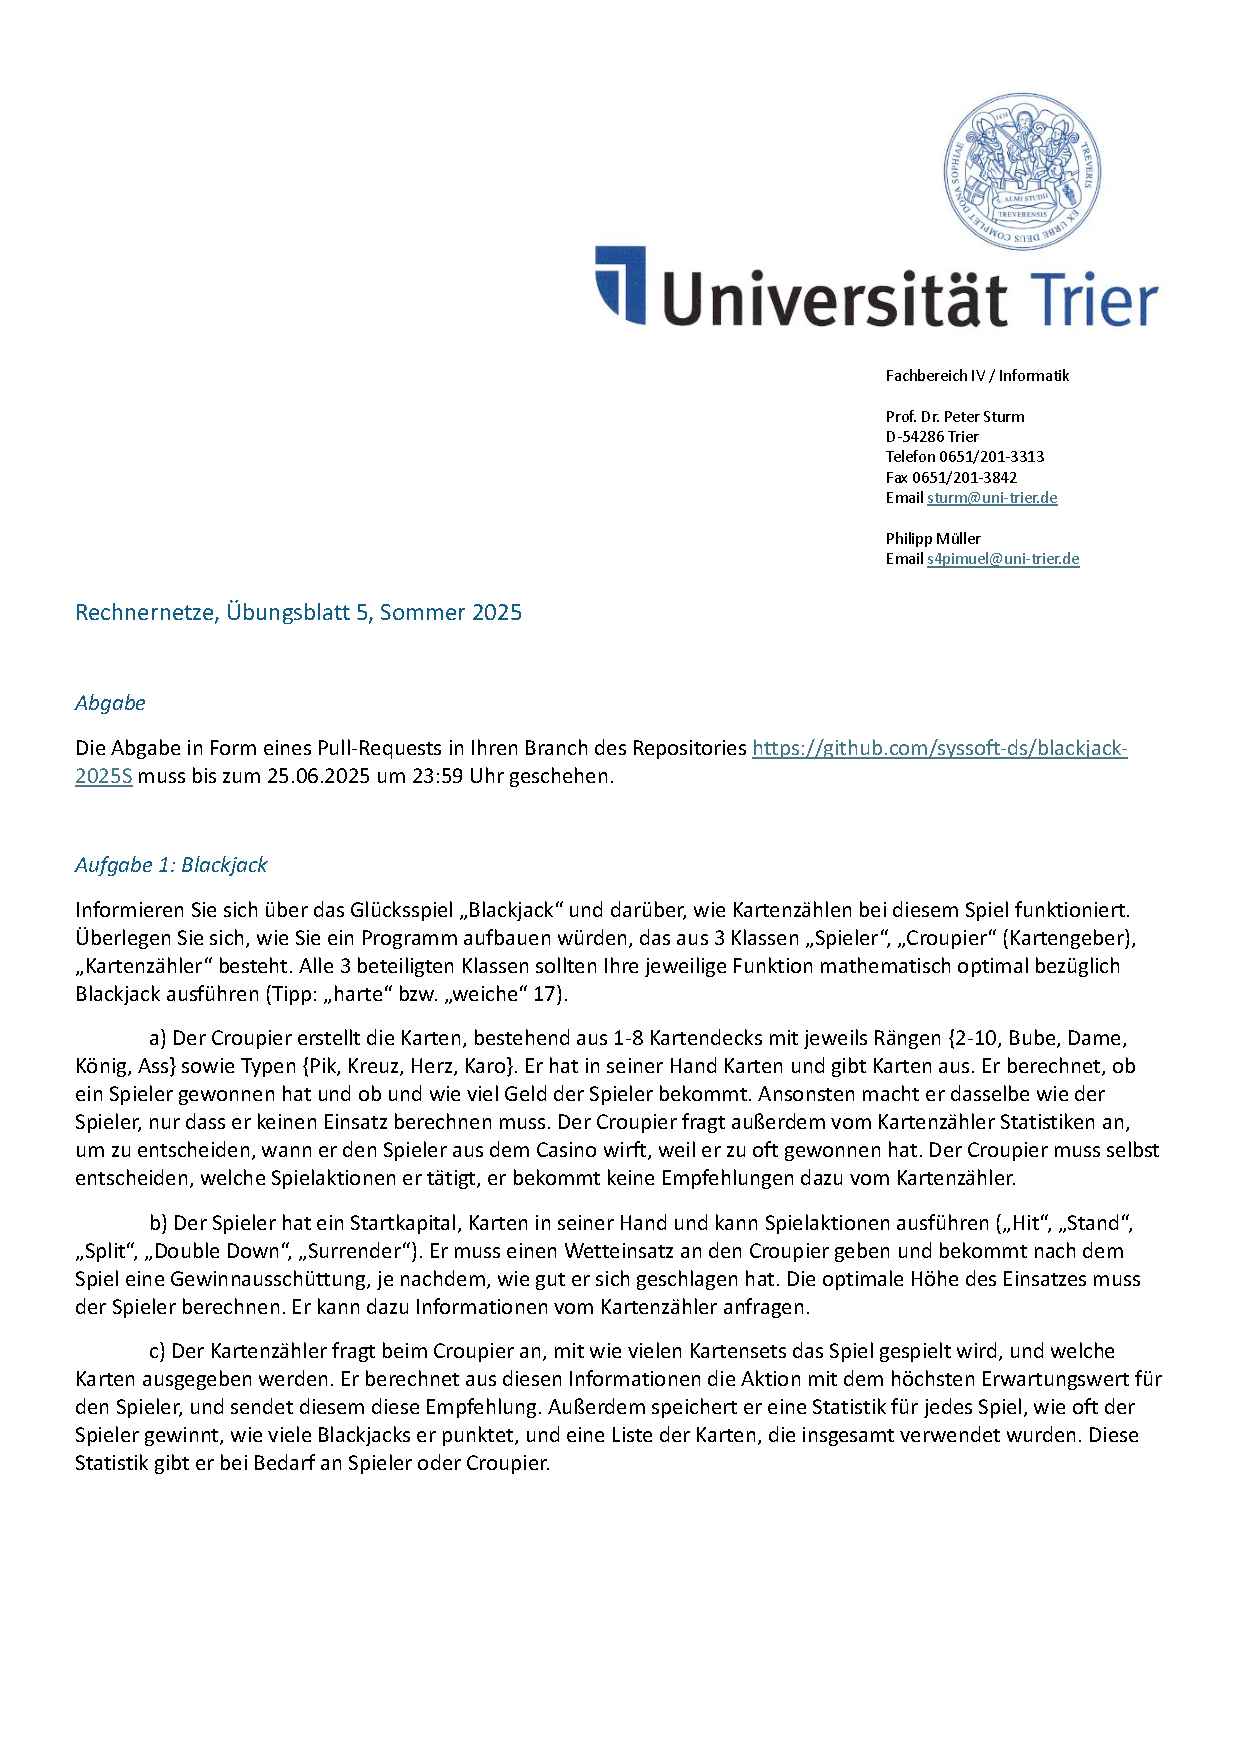
\includepdf[pages=-]{blatt_5/u5.pdf}
	
	\parindent=0cm
	
	\large
	\textbf{Aufgabe 1}\par
	\normalsize
	\vspace{12pt}
	Siehe google docs und Diagramme unter \textit{diagrams/} bzw. \textit{out/}
	\vspace{24pt}
	
	\large
	\textbf{Aufgabe 2}\par
	\normalsize
	\vspace{12pt}
	
	Es muss sichergestellt werden, dass nachrichten, die verschickt werden, ankommen. Das kann durch ein Quittungssystem sichergestellt werden, das für jede versendete spielbezogene Nachricht auf eine Quittung wartet. Damit das jeweilige Programm (Croupier, Kartenzähler oder Spieler) nicht zu lange wartet, sollte weiterhin ein Timeout für die Antwort festgelegt werden. Ferner kann die Kommunikation zwischen den 3 Programmen robuster gemacht werden, indem Nachrichten, die die zulässige Zeit (timeout) überschritten haben, erneut gesendet werden. Dabei sollte einerseits eine maximale Anzahl an \textit{resends} festgelegt werden, z.B. 5 und andererseits sollte die Länge des Timeouts für jeden \textit{resend} erhöht werden.\par
	Um Fehlinterpretationen von Paketen zu vermeiden, sollte eine einheitliche Syntax für den Aufbau der Nachrichten sowie ein einheitliches Format z.B. Json festgelegt werden. ()Siehe google Docs.)\par
	Außerdem soillte ein allgemeiner Programmablauf und die Punkte an denen Nachrichten ausgetauscht sowie welche Nachrichten an diesen Punkten ausgetauscht werden, festgelegt werden. Das verhindert, dass der Programmfluss stecken bleibt, da ein oder mehrere Teilnehmer auf Nachrichten warten, die nicht gesendet werden.\par
	
	\large
	\textbf{Aufgabe 3}\par
	\normalsize
	\vspace{12pt}
	Leider hat sich niemand, der/die einen Kartenzähler implementieren sollten an unserer Diskussion im google Docs beteiligt, entsprechend fehlt die Logik für die Kommunikation mit dieser Klasse / ist nur in Ansätzen in meiner Implementierung der Croupier-Klasse vorhanden.\par
	
	\large
	\textbf{Aufgabe 4}\par
	\normalsize
	\vspace{12pt}
	
	Haben wir gemacht. Waren gefühlt aber auch die einzigen 3 Teilnehmer, die das google Docs genutzt haben. Schade, weil die Aufgabe eigentlich echt Spaß gemacht hat\par. 
	
	\end{document}